% This is samplepaper.tex, a sample chapter demonstrating the
% LLNCS macro package for Springer Computer Science proceedings;
% Version 2.20 of 2017/10/04
%
\RequirePackage{amsmath}
\documentclass[runningheads]{llncs}
%
\usepackage{amssymb}
\usepackage[noend]{algpseudocode} 
\usepackage{algorithm}

\usepackage{tikz}
\usepackage{graphicx}
\newcommand{\acm}[3]{\{#1\}\rightarrow#3}
\newcommand{\ac}[3]{$\{#1\}\rightarrow#3$}
\newcommand{\omesi}{^\omega_\varsigma}
\usepackage{url}
% Macros relatives à la traduction de PH avec arcs neutralisants vers PH à k-priorités fixes

% Macros générales
%\newcommand{\ie}{\textit{i.e.} }
\newcommand{\segm}[2]{\llbracket #1; #2 \rrbracket}
%\newcommand{\f}[1]{\mathsf{#1}}

% Notations générales pour PH
\newcommand{\PH}{\mathcal{PH}}
%\newcommand{\PHs}{\mathcal{S}}
\newcommand{\PHs}{\Sigma}
%\newcommand{\PHp}{\mathcal{P}}
\newcommand{\PHp}{\textcolor{red}{\mathcal{P}}}
%\newcommand{\PHproc}{\mathcal{P}}
\newcommand{\PHproc}{\mathbf{Proc}}
\newcommand{\Proc}{\PHproc}
\newcommand{\PHh}{\mathcal{H}}
\newcommand{\PHa}{\PHh}
%\newcommand{\PHa}{\mathcal{A}}
\newcommand{\PHl}{\mathcal{L}}
\newcommand{\PHn}{\mathcal{N}}

\newcommand{\PHhitter}{\mathsf{hitter}}
\newcommand{\PHtarget}{\mathsf{target}}
\newcommand{\PHbounce}{\mathsf{bounce}}
%\newcommand{\PHsort}{\Sigma}
\newcommand{\PHsort}{\PHs}

%\newcommand{\PHfrappeur}{\mathsf{frappeur}}
%\newcommand{\PHcible}{\mathsf{cible}}
%\newcommand{\PHbond}{\mathsf{bond}}
%\newcommand{\PHsorte}{\mathsf{sorte}}
%\newcommand{\PHbloquant}{\mathsf{bloquante}}
%\newcommand{\PHbloque}{\mathsf{bloquee}}

%\newcommand{\PHfrappeR}{\textcolor{red}{\rightarrow}}
%\newcommand{\PHmonte}{\textcolor{red}{\Rsh}}

\newcommand{\PHhitA}{\rightarrow}
\newcommand{\PHhitB}{\Rsh}
%\newcommand{\PHfrappe}[3]{\mbox{$#1\PHhitA#2\PHhitB#3$}}
%\newcommand{\PHfrappebond}[2]{\mbox{$#1\PHhitB#2$}}
\newcommand{\PHhit}[3]{#1\PHhitA#2\PHhitB#3}
\newcommand{\PHfrappe}{\PHhit}
\newcommand{\PHhbounce}[2]{#1\PHhitB#2}
\newcommand{\PHobj}[2]{\mbox{$#1\PHhitB^*\!#2$}}
\newcommand{\PHobjectif}{\PHobj}
\newcommand{\PHconcat}{::}
%\newcommand{\PHneutralise}{\rtimes}
\def\Sce{\mathbf{Sce}}

% Actions plurielles
\newcommand{\PHhitmultsymbol}{\rightarrowtail}
\newcommand{\PHhitmult}[2]{\mbox{$#1 \PHhitmultsymbol #2$}}
\newcommand{\PHfrappemult}{\PHhitmult}
\newcommand{\PHfrappemults}[2]{\PHhitmult{\{#1\}}{\{#2\}}}

\def\PHget#1#2{{#1[#2]}}
%\newcommand{\PHchange}[2]{#1\langle #2 \rangle}
%\newcommand{\PHchange}[2]{(#1 \Lleftarrow #2)}
%\newcommand{\PHarcn}[2]{\mbox{$#1\PHneutralise#2$}}
\newcommand{\PHplay}{\cdot}

\newcommand{\PHstate}[1]{\mbox{$\langle #1 \rangle$}}
\newcommand{\PHetat}{\PHstate}

\def\supp{\mathsf{support}}
\def\first{\mathsf{first}}
\def\last{\mathsf{last}}

\def\DNtrans{\rightarrow_{ADN}}
\def\DNdef{(\mathbb F, \langle f^1, \dots, f^n\rangle)}
\def\DNdep{\mathsf{dep}}
\def\PHPtrans{\rightarrow_{PH}}
\def\get#1#2{#1[{#2}]}
\def\encodeF#1{\mathbf{#1}}
\def\toPH{\encodeF{PH}}
\def\card#1{|#1|}
\def\decode#1{\llbracket#1\rrbracket}
\def\encode#1{\llparenthesis#1\rrparenthesis}
\def\Hits{\PHa}
\def\hit{\PHhit}
\def\play{\cdot}

\def\Pint{\textsc{PINT}}



\usepackage{ifthen}

\newcommand{\currentScope}{}
\newcommand{\currentSort}{}
\newcommand{\currentSortLabel}{}
\newcommand{\currentAlign}{}
\newcommand{\currentSize}{}

\newcounter{la}
\newcommand{\TSetSortLabel}[2]{
  \expandafter\repcommand\expandafter{\csname TUserSort@#1\endcsname}{#2}
}
\newcommand{\TSort}[4]{
  \renewcommand{\currentScope}{#1}
  \renewcommand{\currentSort}{#2}
  \renewcommand{\currentSize}{#3}
  \renewcommand{\currentAlign}{#4}
  \ifcsname TUserSort@\currentSort\endcsname
    \renewcommand{\currentSortLabel}{\csname TUserSort@\currentSort\endcsname}
  \else
    \renewcommand{\currentSortLabel}{\currentSort}
  \fi
  \begin{scope}[shift={\currentScope}]
  \ifthenelse{\equal{\currentAlign}{l}}{
    \filldraw[process box] (-0.5,-0.5) rectangle (0.5,\currentSize-0.5);
    \node[sort] at (-0.2,\currentSize-0.4) {\currentSortLabel};
   }{\ifthenelse{\equal{\currentAlign}{r}}{
     \filldraw[process box] (-0.5,-0.5) rectangle (0.5,\currentSize-0.5);
     \node[sort] at (0.2,\currentSize-0.4) {\currentSortLabel};
   }{
    \filldraw[process box] (-0.5,-0.5) rectangle (\currentSize-0.5,0.5);
    \ifthenelse{\equal{\currentAlign}{t}}{
      \node[sort,anchor=east] at (-0.3,0.2) {\currentSortLabel};
    }{
      \node[sort] at (-0.6,-0.2) {\currentSortLabel};
    }
   }}
  \setcounter{la}{\currentSize}
  \addtocounter{la}{-1}
  \foreach \i in {0,...,\value{la}} {
    \TProc{\i}
  }
  \end{scope}
}

\newcommand{\TTickProc}[2]{ % pos, label
  \ifthenelse{\equal{\currentAlign}{l}}{
    \draw[tick] (-0.6,#1) -- (-0.4,#1);
    \node[tick label, anchor=east] at (-0.55,#1) {#2};
   }{\ifthenelse{\equal{\currentAlign}{r}}{
    \draw[tick] (0.6,#1) -- (0.4,#1);
    \node[tick label, anchor=west] at (0.55,#1) {#2};
   }{
    \ifthenelse{\equal{\currentAlign}{t}}{
      \draw[tick] (#1,0.6) -- (#1,0.4);
      \node[tick label, anchor=south] at (#1,0.55) {#2};
    }{
      \draw[tick] (#1,-0.6) -- (#1,-0.4);
      \node[tick label, anchor=north] at (#1,-0.55) {#2};
    }
   }}
}
\newcommand{\TSetTick}[3]{
  \expandafter\repcommand\expandafter{\csname TUserTick@#1_#2\endcsname}{#3}
}

\newcommand{\myProc}[3]{
  \ifcsname TUserTick@\currentSort_#1\endcsname
    \TTickProc{#1}{\csname TUserTick@\currentSort_#1\endcsname}
  \else
    \TTickProc{#1}{#1}
  \fi
  \ifthenelse{\equal{\currentAlign}{l}\or\equal{\currentAlign}{r}}{
    \node[#2] (\currentSort_#1) at (0,#1) {#3};
  }{
    \node[#2] (\currentSort_#1) at (#1,0) {#3};
  }
}
\newcommand{\TSetProcStyle}[2]{
  \expandafter\repcommand\expandafter{\csname TUserProcStyle@#1\endcsname}{#2}
}
\newcommand{\TProc}[1]{
  \ifcsname TUserProcStyle@\currentSort_#1\endcsname
    \myProc{#1}{\csname TUserProcStyle@\currentSort_#1\endcsname}{}
  \else
    \myProc{#1}{process}{}
  \fi
}

\newcommand{\repcommand}[2]{
  \providecommand{#1}{#2}
  \renewcommand{#1}{#2}
}
\newcommand{\THit}[5]{
  \path[hit] (#1) edge[#2] (#3#4);
  \expandafter\repcommand\expandafter{\csname TBounce@#3@#5\endcsname}{#4}
}
\newcommand{\TBounce}[4]{
  (#1\csname TBounce@#1@#3\endcsname) edge[#2] (#3#4)
}

%\newcommand{\TState}[1]{
%  \foreach \proc in {#1} {
%    \node[current process] (\proc) at (\proc.center) {};
%  }
%}

\newcommand{\TState}[1]{
  \foreach \proc in {#1} {
        \node[current process] (\proc) at (\proc.center) {};
  };
}
\newcommand{\TCoopHit}[6]{
  \node[#2, apdot] at (#3) {};
  \foreach \proc in {#1} {
    \draw[#2,-] (#3) edge (\proc);
  }
  \path[hit] (#3) edge[#2] (#4#5);
  \expandafter\repcommand\expandafter{\csname TBounce@#4@#6\endcsname}{#5}
}

% ex : \TAction{c_1}{a_1.west}{a_0.north west}{}{right}
% #1 = frappeur
% #2 = cible
% #3 = bond
% #4 = style frappe
% #5 = style bond
\newcommand{\TAction}[5]{
  \THit{#1}{#4}{#2}{}{#3}
  \path[bounce, bend #5=50] \TBounce{#2}{}{#3}{};
}

% ex : \TActionPlur{f_1, c_0}{a_0.west}{a_1.south west}{}{3.5,2.5}{left}
% #1 = frappeur
% #2 = cible
% #3 = bond
% #4 = style frappe
% #5 = coordonnées point central
% #6 = direction bond
\newcommand{\TActionPlur}[6]{
  \TCoopHit{#1}{#4}{#5}{#2}{}{#3}
  \path[bounce, bend #6=50] \TBounce{#2}{}{#3}{};
}

% procedure, abstractions and dependencies
\newcommand{\abstr}[1]{#1^\wedge}%\text{\textasciicircum}}
\def\BS{\mathbf{BSeq}}
\def\aBS{\abstr{\BS}}
\def\abeta{\abstr{\beta}}
\def\aZ{\abstr{\zeta}}
\def\aY{\abstr{\xi}}

\def\beforeproc{\vartriangleleft}

\def\powerset{\wp}

\def\Sce{\mathbf{Sce}}
\def\OS{\mathbf{OSeq}}
\def\Obj{\mathbf{Obj}}
%\def\Proc{\mathbf{Proc}}
%\def\Sol{\mathbf{Sol}}
\newcommand{\Sol}{\mathbf{Sol}}
\newcommand{\NSol}{\Sol}
\newcommand{\sSol}{\mathbf{Sync}}

\usepackage{galois}
\newcommand{\theOSabstr}{toOS}
\newcommand{\OSabstr}[1]{\theOSabstr(#1)}
\newcommand{\theOSconcr}{toSce}
\newcommand{\OSconcr}[1]{\theOSconcr(#1)}

% \def\gO{\mathbb{O}}
% \def\gS{\mathbb{S}}
\def\aS{\mathcal{A}}
\def\Req{\mathrm{Req}}
%\def\Sol{\mathrm{Sol}}
\def\Cont{\mathrm{Cont}}
\def\cBS{\BS_\ctx}
\def\caBS{\aBS_\ctx}
\def\caS{\aS_\ctx}
\def\cSol{\Sol_\ctx}
\def\cReq{\Req_\ctx}
\def\cCont{\Cont_\ctx}

\def\any{\star}

% \def\gProc{\mathrm{maxPROC}}
\def\mCtx{\mathrm{maxCtx}}

%\def\procs{\f{procs}}
\def\objs{\f{objs}}
\def\sat#1{\lceil #1\rceil}

\def\gCont{\f{maxCont}}
\def\lCont{\f{minCont}}
\def\lProc{\f{minProc}}
\def\gProc{\f{maxProc}}

\def\join{\oplus}
\def\concat{\!::\!}
\def\emptyseq{\varepsilon}
\def\ltw{\preccurlyeq_{\OS}}
\def\indexes#1{\mathbb{I}^{#1}}
%\def\indexes#1{\{1..|#1|\}}
\def\supp{\f{support}}
\def\w{\omega}
\def\W{\Omega}
% \def\ctx{\varsigma}
%\def\ctx{{\textcolor{green}{s}}}
% \def\ctx{s}
% \def\Ctx{\mathbf{Ctx}}
\def\Ctx{\mathbf{Ctx}}
\def\mconcr{\gamma}
\def\concr{\mconcr_s}
\def\obj#1#2{{#1\!\Rsh^*\!\!#2}}
\def\objp#1#2#3{\obj{{#1}_{#2}}{{#1}_{#3}}}
\def\A{\mathcal{A}}
\def\cwA{\A_\ctx^\w}
\def\cwReq{\Req_\ctx^\w}
\def\cwSol{\Sol_\ctx^\w}
\def\cwCont{\Cont_\ctx^\w}
\def\gCtx{\f{maxCtx}}
\def\endCtx{\f{endCtx}}
\def\ceil{\f{end}}

%\def\lfp{\mathrm{lfp}\;}
%\def\mlfp#1{\mathrm{lfp}\{#1\}\;}
\newcommand{\lfp}[3]{\mathbf{lfp}\{#1\}\left(#2\mapsto#3\right)}
\def\maxobjs{{\f{maxobjs}}}
\def\maxprocs{{\f{maxprocs}_\ctx}}
\def\objends{{\f{ends}}}

\def\ra{\rho}
\def\rb{\rho^\wedge}
\def\rc{\widetilde{\rho}}
\def\interleave{\f{interleave}}

\def\join{\concat}

\tikzstyle{aS}=[every edge/.style={draw,->,>=stealth}]
\tikzstyle{Asol}=[draw,circle,minimum size=5pt,inner sep=0,node distance=1cm]
\tikzstyle{Aproc}=[draw,node distance=1cm]
\tikzstyle{Aobj}=[node distance=1.5cm]
\tikzstyle{Anos}=[font=\Large]
\tikzstyle{Assol}=[node distance=1.2cm]
%\tikzstyle{AprocPrio}=[Aproc,double]
\tikzstyle{AsolPrio}=[Asol,double]
\tikzstyle{AprocPrio}=[Aproc,double]
\tikzstyle{aSPrio}=[aS,double]


\newcommand{\startl}[1]{\node[Aproc] (#1) {$#1$};\node[Asol,right of=#1] (#1s) {};\path (#1) edge (#1s);}%start link
\newcommand{\link}[2]{\node[Aproc,right of=#1s] (#2) {$#2$};\node[Asol,right of=#2] (#2s) {};\path (#1s) edge (#2) (#2) edge (#2s);} %normal link
\newcommand{\specl}[3]{\node[Aproc,#1 right of=#2s] (#3) {$#3$};\node[Asol,right of=#3] (#3s) {};\path (#2s) edge (#3) (#3) edge (#3s);} %special link
\newcommand{\edl}[2]{\node[Assol,right of=#1s] (#1st){$\varnothing$};\path (#1s) edge (#1st);}%end link


%\def\procs{\mathsf{procs}}
%\def\allprocs{\mathsf{allProcs}}
%\def\allprocs{\procs}
%\def\pfp{\mathsf{pfp}}
\def\pfp{\mathsf{focals}^1}
\def\pfpprocs{\mathsf{pfpProcs}}
\def\bounceprocs{\mathsf{bounceProcs}}
\def\newprocs{\mathsf{newProcs}}

\def\aB{\mathcal{B}}
\def\sat#1{{#1}}
%\def\sat#1{\lceil #1\rceil}
\newcommand{\thisB}[2]{\sat{\aB_{#2}^{#1}}}
\newcommand{\myp}{u}
%\def\cwB{\thisB{\myp}{\ctx}}
\def\cwB{\thisB{\myp}{s}}
%\def\cwB{\sat{\aB_\ctx^\w}}
%\def\cwBz{\thisB{\myp}{\ctx_0}}
\def\cwBz{\thisB{\myp}{s_0}}
\def\mycwB#1#2{\sat{\aB_{#1}^{#2}}}
\def\Bsol{\sat{\Sol^\w_\ctx}}
\def\Breq{\sat{\Req^\w_\ctx}}
\def\Bcont{\sat{\Cont^\w_\ctx}}

\def\myB{\aB^\myp_\ctx}
\def\mysol{\overline{\Sol^\w_\ctx}}
\def\myreq{\overline{\Req^\w_\ctx}}
\def\mycont{\overline{\Cont^\w_\ctx}}

\newcommand{\csState}{\mathsf{procState}}

\newcommand{\V}{V}
\newcommand{\E}{E}
\newcommand{\cwV}{\V_s^\myp}
\newcommand{\cwE}{\E_s^\myp}
% \newcommand{\cwV}{\V_\ctx^\myp}
% \newcommand{\cwE}{\E_\ctx^\myp}
%\newcommand{\VProc}{\textcolor{red}{\V_\PHproc}}
%\newcommand{\VObj}{\textcolor{red}{\V_\Obj}}
%\newcommand{\VSol}{\V_{Sol}}
%\newcommand{\VSol}{\textcolor{red}{\V_{\Sol}}}
\newcommand{\VProc}{\V \cap \PHproc}
\newcommand{\VObj}{\V \cap \Obj}
\newcommand{\VSol}{\V \cap \Sol}
\newcommand{\cwVProc}{\cwV \cap \PHproc}
\newcommand{\cwVObj}{\cwV \cap \Obj}
\newcommand{\cwVSol}{\cwV \cap \Sol}
\newcommand{\cwVsSol}{\cwV \cap \sSol}

\def\Bv{\sat{\cwV}}
\def\Be{\sat{\cwE}}
\def\BvProc{\textcolor{red}{\sat{\cwV}^\PHproc}}
\def\BvObj{\textcolor{red}{\sat{\cwV}^\Obj}}
%\def\BvSol{\sat{\cwV}^{Sol}}
\def\BvSol{\textcolor{red}{\sat{\cwV}^{\Sol}}}

\def\cwBNodes{\Bv}
\def\cwBEdges{\Be}
\def\nsol{\f{nsol}}
\def\conn{\f{conn}}

\newcommand{\Bee}[2]{\Be^{#1}_{#2}}

%\def\mlfp#1{\f{pppf}\{#1\}}

\def\PHobjp#1#2#3{\PHobj{{#1}_{#2}}{{#1}_{#3}}}
\def\Obj{\mathbf{Obj}}
\def\powerset{\wp}
\def\gCont{\f{maxCont}}

\def\muconcr{\ell}
\def\uconcr{\muconcr_\ctx}

% Styles TikZ et couleurs personnalisées

\usepackage{tikz}

\newdimen\pgfex
\newdimen\pgfem
\usetikzlibrary{arrows,shapes,shadows,scopes}
\usetikzlibrary{positioning}
\usetikzlibrary{matrix}
\usetikzlibrary{decorations.text}
\usetikzlibrary{decorations.pathmorphing}
\usetikzlibrary{arrows,shapes}

\definecolor{lightgray}{rgb}{0.8,0.8,0.8}
\definecolor{lightgrey}{rgb}{0.8,0.8,0.8}

\definecolor{lightred}{rgb}{1,0.8,0.8}
\definecolor{lightgreen}{rgb}{0.7,1,0.7}
\definecolor{darkgreen}{rgb}{0,0.5,0}
\definecolor{darkblue}{rgb}{0,0,0.5}
\definecolor{darkyellow}{rgb}{0.5,0.5,0}
\definecolor{lightyellow}{rgb}{1,1,0.6}
\definecolor{darkcyan}{rgb}{0,0.6,0.6}
\definecolor{lightcyan}{rgb}{0.6,1,1}
\definecolor{darkorange}{rgb}{0.8,0.2,0}
\definecolor{notsodarkred}{rgb}{0.8,0,0}

\definecolor{notsodarkgreen}{rgb}{0,0.7,0}

%\definecolor{coloract}{rgb}{0,1,0}
%\definecolor{colorinh}{rgb}{1,0,0}
\colorlet{coloract}{darkgreen}
\colorlet{colorinh}{red}
\colorlet{coloractgray}{lightgreen}
\colorlet{colorinhgray}{lightred}
\colorlet{colorinf}{darkgray}
\colorlet{coloractgray}{lightgreen}
\colorlet{colorinhgray}{lightred}

\colorlet{colorgray}{lightgray}
\colorlet{colorhl}{blue}


\tikzstyle{boxed ph}=[]
\tikzstyle{sort}=[fill=lightgray, rounded corners, draw=black]
\tikzstyle{process}=[circle,draw,minimum size=15pt,fill=white,font=\footnotesize,inner sep=1pt]
%\tikzstyle{black process}=[process, draw=blue, fill=red,text=black,font=\bfseries]
\tikzstyle{gray process}=[process, draw=black, fill=lightgray]
\tikzstyle{highlighted process}=[current process, fill=gray]
\tikzstyle{process box}=[fill=none,draw=black,rounded corners]
\tikzstyle{current process}=[process, draw=black, fill=lightgray]
%\tikzstyle{current process}=[process,fill=lightcyan]
\tikzstyle{hl process}=[process,fill=blue!30]
\tikzstyle{tick label}=[font=\footnotesize]
\tikzstyle{tick}=[densely dotted] %-
\tikzstyle{hit}=[->,>=angle 45]
\tikzstyle{selfhit}=[min distance=50pt,curve to]
\tikzstyle{bounce}=[densely dotted,>=stealth',->]
\tikzstyle{ulhit}=[draw=lightgray,fill=lightgray]
\tikzstyle{pulhit}=[fill=lightgray]
\tikzstyle{bulhit}=[draw=lightgray]
\tikzstyle{hl}=[very thick,colorhl]
\tikzstyle{hlb}=[very thick]
\tikzstyle{hlhit}=[hl]
%\tikzstyle{hl2}=[hl]
%\tikzstyle{nohl}=[font=\normalfont,thin]

\tikzstyle{update}=[draw,->,dashed,shorten >=.7cm,shorten <=.7cm]

\tikzstyle{unprio}=[draw,thin]%[double]
%\tikzstyle{prio}=[draw,thick,-stealth]%[double]
\tikzstyle{prio}=[draw,-stealth,double]

\tikzstyle{hitless graph}=[every edge/.style={draw=red,-}]

\tikzstyle{aS}=[every edge/.style={draw,->,>=stealth}]
\tikzstyle{Asol}=[draw,circle,minimum size=5pt,inner sep=0,node distance=1cm]
\tikzstyle{Aproc}=[draw,node distance=1.2cm]
\tikzstyle{Aobj}=[node distance=1.5cm]
\tikzstyle{Anos}=[font=\Large]

\tikzstyle{AsolPrio}=[Asol,double]
\tikzstyle{AprocPrio}=[Aproc,double]
\tikzstyle{aSPrio}=[aS,double]

\colorlet{colorhlwarn}{notsodarkred}
\colorlet{colorhlwarnbg}{lightred}
\tikzstyle{Ahl}=[very thick,fill=colorhlwarnbg,draw=colorhlwarn,text=colorhlwarn]
\tikzstyle{Ahledge}=[very thick,double=colorhlwarnbg,draw=colorhlwarn,color=colorhlwarn]





%\definecolor{darkred}{rgb}{0.5,0,0}



\tikzstyle{grn}=[every node/.style={circle,draw=black,outer sep=2pt,minimum
                size=15pt,text=black}, node distance=1.5cm, ->]
\tikzstyle{inh}=[>=|,-|,draw=colorinh,thick, text=black,label]
\tikzstyle{act}=[->,>=triangle 60,draw=coloract,thick,color=coloract]
\tikzstyle{inhgray}=[>=|,-|,draw=colorinhgray,thick, text=black,label]
\tikzstyle{actgray}=[->,>=triangle 60,draw=coloractgray,thick,color=coloractgray]
\tikzstyle{inf}=[->,draw=colorinf,thick,color=colorinf]
%\tikzstyle{elabel}=[fill=none, above=-1pt, sloped,text=black, minimum size=10pt, outer sep=0, font=\scriptsize,draw=none]
\tikzstyle{elabel}=[fill=none,text=black, above=-2pt,%sloped,
minimum size=10pt, outer sep=0, font=\scriptsize, draw=none]
%\tikzstyle{elabel}=[]


\tikzstyle{plot}=[every path/.style={-}]
\tikzstyle{axe}=[black,->,>=stealth']
\tikzstyle{ticks}=[font=\scriptsize,every node/.style={black}]
\tikzstyle{mean}=[thick]
\tikzstyle{interval}=[line width=5pt,red,draw opacity=0.7]
%\definecolor{lightred}{rgb}{1,0.3,0.3}

%\tikzstyle{hl}=[yellow]
%\tikzstyle{hl2}=[orange]

%\tikzstyle{every matrix}=[ampersand replacement=\&]
%\tikzstyle{shorthandoff}=[]
%\tikzstyle{shorthandon}=[]
\tikzstyle{objective}=[process,very thick,fill=yellow!50]

\tikzstyle{coopupdate}=[-stealth,decorate,decoration={zigzag,amplitude=1.5pt,post=lineto,post length=.3cm,pre=lineto,pre length=.3cm}]

\tikzstyle{labelprio}=[circle, fill=blue!30, inner sep=0pt, minimum size=13pt]
\tikzstyle{labelprio1}=[labelprio]
\tikzstyle{labelprio2}=[labelprio, fill=red!60]
\tikzstyle{labelprio3}=[labelprio, fill=orange!50]
\tikzstyle{labelprio4}=[labelprio, fill=brown!50]

\tikzstyle{labelstocha}=[rectangle, rounded corners=4pt]

\tikzstyle{andot}=[circle, fill=black, inner sep=1.2pt, draw=transparent]
\tikzstyle{anligne}=[thick]

\tikzstyle{apdot}=[andot] %[circle, fill=black, draw=black, inner sep=1]
\tikzstyle{apdotsimple}=[] %[circle, fill=black, draw=black, inner sep=1]

% Figure de résumé des liens entre les formalismes
\tikzstyle{equiv-externe}=[thick, rounded corners, draw=gray, fill=gray!10, align=center,
  inner sep=8]

% label pour les délais des actions 
 \tikzstyle{labeldelai1}=[circle, fill=red!60, inner sep=0pt, minimum size=8pt]
  \tikzstyle{labeldelai2}=[circle, fill=blue!30, inner sep=0pt, minimum size=8pt]
  \tikzstyle{labeldelai3}=[circle, fill=brown!50, inner sep=0pt, minimum size=8pt]
  \tikzstyle{labeldelai4}=[circle, fill=green!50, inner sep=0pt, minimum size=8pt]
  
% Automata Networks:
\tikzstyle{local transitions}=[->,>=latex',thick,bend left=30,
               every node/.style={fill=white,inner sep=1pt,outer sep=1pt}]
\tikzstyle{reach}=[fill=lightgray,ellipse]

\tikzstyle{local transitions 2}=[->,>=latex',thick,bend left=100,
               every node/.style={fill=white,inner sep=1pt,outer sep=4pt}]

\tikzstyle{local transitions 3}=[->,>=latex',thick,bend right=100,
               every node/.style={ right, fill=white,inner sep=1pt,outer sep=4pt}]
               
% Graphe d'états
% noeuds
\tikzstyle{vide}= [rectangle, minimum width=2em,minimum height=1.5em,]
\tikzstyle{stable}= [rectangle,fill=lightred]
\tikzstyle{current}= [rectangle,fill=lightcyan]
\tikzstyle{initial}= [rectangle,fill=green!20]

% % STG transitions
\tikzstyle{etiquette}=[midway,fill=blue!20,circle,scale=0.7pt]
\tikzstyle{etiquette2}=[midway,fill=green!20,circle,scale=0.7pt]
%
\tikzstyle{currentTrans}=[->,very thick,blue]
\tikzstyle{seperatedTransPart1}=[draw, thick, blue]
\tikzstyle{seperatedTransPart2}=[->, thick, blue]


\tikzstyle{mytext}=[thick, text width=4.5em,inner sep=1pt]
\tikzstyle{line} =[draw, thick, -latex',shorten >=2pt]
\tikzstyle{block} =[rectangle,text width=6em,draw,minimum height=4em, outer sep=0pt]

\tikzstyle{adn}=[every node/.style={circle,draw=black,outer sep=2pt,minimum
                size=15pt,text=black}, node distance=1.5cm, ->]
                
% Définition des nouvelles options xmin, xmax, ymin, ymax
% Valeurs par défaut : -3, 3, -3, 3
\tikzset{
    xmin/.store in=\xmin, xmin/.default=-3, xmin=-3,
    xmax/.store in=\xmax, xmax/.default=3, xmax=3,
    ymin/.store in=\ymin, ymin/.default=-3, ymin=-3,
    ymax/.store in=\ymax, ymax/.default=3, ymax=3,
}
% Commande qui trace la grille entre (xmin,ymin) et (xmax,ymax)
\newcommand {\grille}
    {\draw[help lines] (\xmin,\ymin) grid (\xmax,\ymax);}
% Commande \axes
\newcommand {\axes} {
    \draw[->] (\xmin,0) -- (\xmax+0.5,0);
    \draw[->] (0,\ymin) -- (0,\ymax+0.5);
}
% Commande qui limite l’affichage à (xmin,ymin) et (xmax,ymax)
\newcommand {\fenetre}
    {\clip (\xmin,\ymin) rectangle (\xmax,\ymax);}
   
 \newcommand{\nombresCopiesParNote}
   {(0,0)(1,0)(2,2)(3,0)(4,6)(5,4)(6,7)(7,4)(8,3)(9,0)(10,1)}  
% Expression level of a
 \newcommand{\expressionDiscreteA}
   {(0,0)(1,0)(2,0)(3,0)(4,0)(4,1)(5,1)(5,0)(6,0)(7,0)(8,0)(9,0)(9,1)(10,1)(11,1)(12,1)(13,1)(13,0)(14,0)(15,0)(16,0)(17,0)(17,1)(18,1)}      
   
% Expression level of b
 \newcommand{\expressionDiscreteB}
   {(0,1)(12,1)(12,0)(18,0)} 
   
% Expression level of z
 \newcommand{\expressionDiscreteZ}
   {(0,0)(3,0)(3,1)(14,1)(14,0)(18,0)}
% Used for displaying a sample figure. If possible, figure files should
% be included in EPS format.
%
% If you use the hyperref package, please uncomment the following line
% to display URLs in blue roman font according to Springer's eBook style:
\renewcommand\UrlFont{\color{blue}\rmfamily}

\begin{document}
%
\title{A Heuristic for Reachability Problem in Asynchronous Binary Automata Networks\thanks{Supported by Laboratoire des Sciences du Num\'erique de Nantes and China Scholarship Council}}
%
\titlerunning{A Heuristic for Reachability Problem}
% If the paper title is too long for the running head, you can set
% an abbreviated paper title here
%
\author{Xinwei Chai \and Morgan Magnin \and Olivier Roux}
%
\authorrunning{X. Chai et al.}
% First names are abbreviated in the running head.
% If there are more than two authors, 'et al.' is used.
%
\institute{Laboratoire des Sciences du Num\'erique de Nantes, UMR CNRS 6004 \'Ecole Centrale de Nantes, 1 rue de la No\"e - B.P. 92101 - 44321 Nantes Cedex 3, France \\
\email{\{xinwei.chai, morgan.magnin, olivier.roux\}@ls2n.fr}}
%
\maketitle              % typeset the header of the contribution
%
\begin{abstract}
On the demand of efficient reachability analysis due to the inevitable complexity of large-scale biological models, this paper is dedicated to a novel approach: PermReach, for reachability problem of our new framework, Asynchronous Binary Automata Networks (ABAN). 
ABAN is an expressive modeling framework which contains all the dynamics behaviors performed by Asynchronous Boolean Networks. 
Compared to Boolean Networks (BN), ABAN has a finer description of state transitions (from a local state to another, instead of symmetric Boolean functions). 
To analyze the reachability properties on large-scale models (like the ones from systems biology), previous works have exhibited an efficient abstraction technique called Local Causality Graph (LCG).
However, this technique may be not conclusive. Our contribution here is to extend these results by tackling those complex intractable cases \textit{via} a heuristic technique. 
To validate our method, tests were conducted in large biological networks and randomly generated examples, showing that our method is more conclusive and faster than existing ones.

\keywords{Asynchronous Binary Automata Networks \and Simplified Local Causality Graph \and Heuristics.}
\end{abstract}
\section{Introduction}
\label{intro}
Works on concurrent systems have been of interest for systems biology for a decade \cite{bockmayr2002using,bortolussi2008modeling,wiley2003computational}. 
In this context, the challenges nowadays consist of not only model validation with regard to existing knowledge on systems but also behavior prediction of these systems. 
%In this context, reachability issue on formal models is a critical challenge which not only validates models with regard to existing knowledge on systems, but also addresses predictions of the behavior of these systems.
With quantities of available data provided by new technologies, \textit{e.g.} DNA microarray \cite{marx2013}, there is a growing need for high-performance analytic tools, especially for reachability problem, as many static and dynamical properties are transformable to the reachability of certain states.
Reachability problem has been studied under many different modeling frameworks for decades \cite{akutsu2007control,barrett2006complexity,Daws1998,esparza1998,mayr1984,wozna2003} and takes an important part in Model Checking \cite{clarke20142}. 
State Space Explosion problem arises in reachability analysis of concurrent systems as the state space is exponential to the number of components in the model, thus disables naive approaches. 

Related studies have been carried over various frameworks: Plateau et al. \cite{plateau1991stochastic} propose a Stochastic Automata Network and study its steady-state behavior, while the reachability analysis is absent; Li et al. \cite{li2012reachability,li2014stability} investigate theoretically the stability, controllability and reachability of Switched Boolean Networks, but their method remains computationally expensive.  
To tackle the State Space Explosion problem, symbolic model checking \cite{burch1992symbolic} and SAT-solvers \cite{abdulla2000symbolic} have been considered over years, but the solution space of original problem remains huge.
Paulev\'e \textit{et al.} \cite{folschette2015,pauleve2011} have proposed Automata Network (AN) for modeling concurrent systems. 
They provide an approach to address this issue by designing a static abstraction (with an over-approximation and an under-approximation of the real dynamics) inspired by abstract interpretation: Local Causality Graph (LCG). 
This static analysis drastically reduces the state-space and avoids costly global search \cite{pauleve2012}.

With the initiative of LCG, this paper is devoted to the study of general reachability problems in Asynchronous Binary Automata Networks (ABAN), then to gain a more profound understanding of the dynamics of biological systems. 
Many biological networks are encoded in Boolean style \cite{kauffman1969}, because BN is a simple formalism but with strong expressiveness also due to the imprecision of raw data.
However BN may be not expressive enough.
To model the dynamic behavior ``$a\gets$ $1$ when $b=1$'', one has $a(t+1)=b(t)$ in BN.
$a$ always follows the evolution of $b$ but with an unwanted behavior ``$a\gets 0$ when $b=0$''.
ABAN models this dynamics as \textit{via} \ac{b_1}{a_0}{a_1} without redundancy. 
Besides, BNs are transformable to Automata Networks, and this property makes ABAN more extendable (Appendix \ref{appendix:C}).

In many circumstances, LCG is able to give a conclusive result on the reachability of target states in polynomial time to the number of automata \cite{pauleve2016goal}. 
However there exists inconclusive cases which disable the reasoning of sufficient conditions.
After diving into the mechanics of LCG and the inconclusive cases, we figure out why those cases are intractable by pure static analysis. 
We develop a heuristic technique aiming at the application for general instances. 
This heuristic method has a better performance on conclusiveness than static reasoning, because it attempts to explore a part of the system dynamics \textit{via} partial verification.
In the end, we conduct tests on signaling networks of around 100 components (TCR and EGFR, see Section \ref{sect:5}): the results of LCG contain inconclusive instances \cite{folschette2015} while our new method solves them.

This paper is organized as follows: in section 2, we will introduce the formal background, Asynchronous Binary Automata Network (ABAN); section 3 presents the analysis of dynamics using only static reasoning; 
section 4 is the core content of this paper, concerning the solution of inconclusive cases; discussion about tests and conclusion are placed in section 5 and 6. \textcolor{red}{To revise at last}

\section{Preliminaries}\label{sect:2}
\textit{Notations}:
\textcolor{red}{verify if they are all used or add some new}
$::$ sequential connector;
$\#$ cardinal;
$a.$next the successor of $a$. 

Asynchronous Binary Automata Network (ABAN) is a variant of traditional AN.
Binary means that every automaton has exactly two possible states $(0,1)$ and asynchronous implies the update scheme with no more than one automaton can change its value at a time. 

\begin{definition}[ABAN]
An ABAN is a triplet $AB = (\mathbf{\Sigma},\mathbf{L},\mathbf{T})$, where:
\begin{itemize}
\item $\mathbf{\Sigma}\triangleq\{a,b,\ldots\}$ is the finite set of automata with every component possessing a Boolean state;
\item $L_a\triangleq\{a_0,a_1\}$ is the set of Boolean states of automaton $a\in \mathbf{\Sigma}$, $\mathbf{LS}\triangleq \underset{a\in \mathbf{\Sigma}}{\cup} L_a$ is the set of all local states,  $\mathbf{L}\triangleq \underset{a\in \mathbf{\Sigma'}}{\times} L_a$ is the set of joint states where $\mathbf{\Sigma'}\subseteq\mathbf{\Sigma}$. Particularly, if $\mathbf{\Sigma'}=\mathbf{\Sigma}$, $\mathbf{L}$ is the set of global states. 
The state of automaton $a$ at state $s$ is denoted $s[a]=a_i$;
\item $\mathbf{T}\subseteq \{A\to b_{i}\mid b\in \mathbf{\Sigma} \land A\in \mathbf{L}\}$ is the set of transitions, where $A$ is the set of required states for the transition, which allows to flip $b_{1-i}$ to $b_i$. $A$ is called head and $b_i$ is called body.
\end{itemize}
\end{definition}

\begin{definition}[Dynamics]
    From global state $s$, the global state after firing transition $tr=A\to b_i$ is denoted $s \cdot tr = (s \setminus \{b_{1-i}\}) \cup \{b_{i}\}, b_{1-i} \in s$.
    The state of a certain automaton $a$ is noted $(s\cdot tr)[a]$.
\end{definition}
To describe the evolution of an ABAN, we use the notion of trajectory:
\begin{definition}[Trajectory]
Given ABAN $AB = (\mathbf{\Sigma},\mathbf{L},\mathbf{T})$ and a global initial state $\alpha\in \mathbf{L}$, a trajectory $t$ from $\alpha$ is a sequence of transitions $t=tr_1::\cdots :: tr_i::\cdots ::tr_n$ with $tr_i\in\mathbf{T}$ and each $tr_i$ is firable in $(\alpha \cdot tr_1 \cdot \ldots \cdot tr_{i-1})$.
From $\alpha$, the global state after firing all transitions of $t$ is denoted $\alpha \cdot t$.
\end{definition}

%From a given initial state $\alpha$, the state after firing $\delta$ is denoted $\alpha\cdot \delta$ and its local form of certain automaton $a$ is noted $(\alpha\cdot \delta)[a]$.
\begin{definition}[Reachability]
Given an global initial state $\alpha$, global state $\Omega$ is reachable iff there exists a trajectory $\delta$ such that $\alpha\cdot \delta=\Omega$, denoted $reach(\alpha, \Omega)$, taking Boolean value $\mathbf{True}$ or $\mathbf{False}$.
Likewise, local state $\omega=a_i$ is reachable iff there exists a trajectory $\delta$ such that $(\alpha\cdot \delta)[a]=a_i$, denoted $reach(\alpha, \omega)$.
\end{definition}
\begin{example}\label{example:aban}
Fig. \ref{fig:1} shows an ABAN with initial state $\alpha=\langle a_0,b_0,c_0,d_0,e_0\rangle$ and a possible trajectory from $\alpha$: $\delta=\acm{d_0}{b_0}{b_1}::\acm{b_1}{d_0}{d_1}::\acm{d_1}{c_0}{c_1}::\acm{b_1,c_1}{a_0}{a_1}$. After firing $\delta$, final state $\Omega=\alpha\cdot \delta=\langle a_1,b_1,c_1,d_1,e_0\rangle$.
$\Omega=\langle a_1,b_1,c_1,d_1,e_0\rangle$ or $\omega=a_1$ is said reachable from $\alpha$ \textit{via} trajectory $\delta$, that is $reach(\alpha,a_1)=\mathbf{True}$ and $reach(\alpha,\Omega)=\mathbf{True}$.
\end{example}
\begin{figure}[ht]
\centering
\begin{tikzpicture}[apdotsimple/.style={apdot},scale=0.7, every node/.style={scale=0.8}]
\scriptsize
\TSort{(0,0)}{a}{2}{l}
\TSort{(2,0)}{b}{2}{l}
\TSort{(4,0)}{c}{2}{l}
\TSort{(6,0)}{d}{2}{l}
\TSort{(8,0)}{e}{2}{l}

% with delays
\path[local transitions]

	(a_0) edge node[auto] {\{$b_1, c_1$\}} (a_1)
    (a_0) edge[bend right] node[right] {$\{e_1\}$} (a_1)
	(b_0) edge node[auto] {$\{d_0\}$} (b_1)
	(d_0) edge node[auto] {$\{b_1\}$} (d_1)
	%(c_1) edge node[auto] {$\{b_0\}$, $2$} (c_0)
	(c_0) edge node[auto] {$\{d_1\}$} (c_1)
;

\TState{a_0, b_0, c_0, d_0,e_0}


\end{tikzpicture}

\caption{Example of ABAN, where circles stand for Boolean states within an automaton and gray ones are initial states.}\label{fig:1}
\end{figure}	

To simplify the notations, all the initial states of ABAN are set to 0 by default.
\section{Static analysis of reachability property}\label{sect:3}
To approach various dynamical properties of such networks, Local Causality Graph (LCG) is an efficient static analytic tool for reachability put forward by Paulev\'e \textit{et al.} \cite{pauleve2011}. 
LCG determines the existence of trajectory of the desired state without traversing the whole state space.

LCG functions as follows: its over-approximation and under-approximation which give respectively a necessary condition and a sufficient condition of reachability. 
With these conditions, we can conclude in many cases.

More importantly, LCG is also able to provide one with a trajectory if $\omega_i$ is reachable suggested by under-approximation.
We are not going to detail the original version of this trajectory finding technique, instead, we propose its adaptation for ABAN in order to approach the solution of inconclusive cases.
In this paper, only binary networks are studied, so we propose a simplified form of LCG instead of two LCGs (over and under-approximation) which is well suited for the present need.
The drawback is also clear: there are inconclusive cases, which means LCG is neither able to solve in this situation, nor able to generate a trajectory (if reachable).
To improve the conclusiveness of this method, we simplified the LCG for over-approximation for binary situations, called SLCG.

To give LCG a wider applicability, in Appendix \ref{appendix:C}, any BN is transformable to ANs and then SLCG is applicable to its analyses of dynamical properties.
\subsection{Simplified Local Causality Graph (SLCG)}
\begin{definition}[SLCG]\label{defSLCG}
Given an ABAN $AB =(\mathbf{\Sigma},\mathbf{L},\mathbf{T})$, an initial state $\alpha$ and a target state $\omega$, SLCG $l=(V_{\mathrm{state}},V_{\mathrm{solution}},E)$ is the smallest recursive structure with $E \subseteq(V_{\mathrm{state}}\times V_{\mathrm{solution}})\cup(V_{\mathrm{solution}}\times V_{\mathrm{state}})$ which satisfies:
\begin{eqnarray*}
    \omega&\in& V_{\mathrm{state}} \\
    a_i\in V_{\mathrm{state}} &\Leftrightarrow& \{(a_i, sol_{a_i})| a_i\in \alpha\}\subseteq E \\
    sol_{a_i}\in V_{\mathrm{solution}}&\Leftrightarrow& \{(sol_{a_i},\mathbf{V}_a(sol_{a_i})\}\subseteq E
\end{eqnarray*}
where $V_{\mathrm{state}}\subseteq\mathbf{LS}$ is the set of states, $V_{\mathrm{solution}}\subseteq \mathbf{T}$ is the set of solutions and $\mathbf{V}_a$ is the set of required local states of $sol_{a_i}$.
\end{definition}
Intuitively, when the recursive construction is complete, SLCG is in fact a digraph with state nodes $V_{\mathrm{state}}$ and solution nodes $V_{\mathrm{solution}}$. 
$E$ consists of the edges between state nodes and solution nodes. 
To access certain local states, at least one of its successive solution (corresponding transitions from solution nodes) needs to be fired; to make one solution node firable, all of its successive local states need to be satisfied. 
A recursive reasoning of reachability begins with a state node representing desired local state, goes through $a_i\mapsto sol_{a_i}\mapsto b_j \cdots$ and ends with initial state (possibly reachable) or a local state without solution successor (unreachable). 
With SLCG, one can compute the pseudo-reachability of a local state, which is a necessary condition of reachability.

\begin{definition}[Pseudo-reachability]\label{defPseudoReach}
Given an SLCG $l=(V_{\mathrm{state}},V_{\mathrm{solution}},E)$ with initial state $\alpha$, the pseudo-reachability of node $v\in V_{\mathrm{state}}$ is defined as
\begin{equation}
\nonumber
    r'(\alpha,v)=
    \begin{cases}
    \mathrm{\bf True} & {\rm if\ } v\in \alpha\\
    \mathrm{\bf False} & {\rm if\ } v\not\in \alpha\ {\rm and} \not\exists(s,sol) \in E\\
    %\bigvee_{(s,sol) \in E} \mathrm{firable}(sol) & otherwise
    \bigvee_{(s,sol) \in E} (\bigwedge_{(sol,s)\in E} r'(\alpha,s)) & {\rm otherwise}
\end{cases}
\end{equation}
%where $\mathrm{firable}(sol)=\bigwedge_{(sol,s)\in E} r'(\alpha,s)$. 

\end{definition}
\begin{example}
In Fig \ref{fig:2}, the left solution node of $a_1$ is not useful because its successor $e_1$ does not have any successive solution node, \textit{i.e.} $e_1$ is unreachable;
the right solution node of $a_1$ requires $b_1$ and $c_1$, they finally lead to $d_0$ then to $\varnothing$.
\textit{i.e.} nothing is needed to reach $d_0$ as $d_0$ appears in the initial state (trivial solution).
One can figure out state nodes act as OR gates while solution nodes act as AND gates. The pseudo-reachability $r'(\alpha,a_1)$ is computed recursively as follows:
\begin{align*}
r'(\alpha,a_1)&=r'(\alpha,e_1)\lor(r'(\alpha,b_1)\land r'(\alpha,c_1))\\
&=r'(\alpha,b_1)\land r'(\alpha,d_1)=r'(\alpha,b_1)=r'(\alpha,d_0)=\mathbf{True}
\end{align*}
\end{example}

\begin{figure}[ht]
\centering
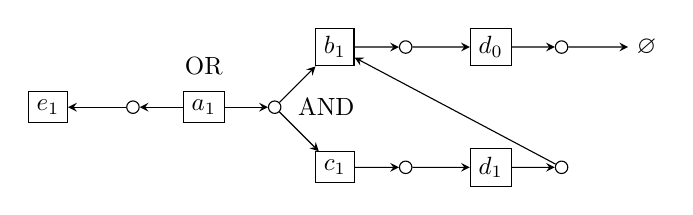
\begin{tikzpicture}[aS,scale=0.9, every node/.style={scale=0.9}]  
  	
  	\startl{a_1};
    \node[Asol,left of=a_1] (a_1s1){};
    \node[Aproc,left of=a_1s1] (e_1){$e_1$};
    \node[right = 0.1cm of a_1s] {AND};
    \node[above = 0.1cm of a_1] {OR};
    \path 
    (a_1s1) edge (e_1)
    (a_1) edge (a_1s1)
    ; 
  	\specl{above}{a_1}{b_1};
  	\link{b_1}{d_0};
  	\edl{d_0};
  	\specl{below}{a_1}{c_1};
	\link{c_1}{d_1};
    \path (d_1s) edge (b_1);
    \end{tikzpicture}

\caption{SLCG showing the local causality of $a_1$ of the ABAN in Fig \ref{fig:1}, with the squares representing local states and small circles representing solution nodes}
\label{fig:2}
\end{figure}

The algorithm of SLCG construction is in Appendix \ref{appendix:B}.

\subsection{Limitation of SLCG}\label{limitation}
Although SLCG allows one to reason the pseudo-reachability locally without traversing the whole state space, it is not equivalent to the reachability if there exists the following structures:
\begin{enumerate}
\item Cycles in SLCG
\item Conflicts in SLCG

\end{enumerate}
To be more formal, a cycle (1) is in the form of $a_i\mapsto\cdots\mapsto a_i$, i.e. to access $a_i$, one has to reach first $a_i$. This self-involvement makes the reachability inconclusive. 
A conflict (2) is that a solution node has multiple successors generating branches, and there are different states of the same automaton \textit{i.e.} $a_i$ and $a_{1-i}$. 
We can not decide the order of reaching these states, because reaching one local state may disable the reachability of another one.
Sometimes there exists a trajectory which accesses these states in certain order, sometimes there does not exist such.

In the following examples, if we ignore those limitations, SLCG does not imply real reachability.


\begin{example}\label{example:reach}
In Fig \ref{fig:1} and 
Fig \ref{fig:2}, although there is a conflict, $a_1$ is reachable.
\end{example}

\begin{example}\label{example:unreach}
In Fig. \ref{fig:3}, $\mathbf{\Sigma}=\{a,b,c\}$, $\mathbf{T}=\{\acm{b_0}{a_0}{a_1},\ \acm{a_0}{b_0}{b_1},\ \acm{\{a_1,b_1\}}{c_0}{c_1}\}$,  desired final state $\omega=a_1$. 
Both $a_1$ and $b_1$ are reachable, but they can not be reached simultaneously.
In the SLCG, there are two branches, $a_1\mapsto b_0$ and $b_1\mapsto a_0$.
Automata $a$ and $b$ involve themselves in different branches, reaching one of them disables the reachability of another one.
\end{example}

\begin{figure}[ht]
\centering
\begin{minipage}{0.4\textwidth}
\centering
\begin{tikzpicture}[apdotsimple/.style={apdot},scale=0.9, every node/.style={scale=0.9}]
\scriptsize
\TSort{(0,0)}{a}{2}{l}
\TSort{(2,0)}{b}{2}{l}
\TSort{(4,0)}{c}{2}{l}

% with delays
\path[local transitions]

	(c_0) edge node[auto] {\{$a_1, b_1$\}} (c_1)
	(a_0) edge node[auto] {\{$b_0$\}} (a_1)
	(b_0) edge node[auto] {\{$\mathbf{a_0}$\}} (b_1)
;
\TState{a_0, b_0, c_0}
\end{tikzpicture}
\end{minipage}\hfill
\begin{minipage}{0.6\textwidth}
\centering
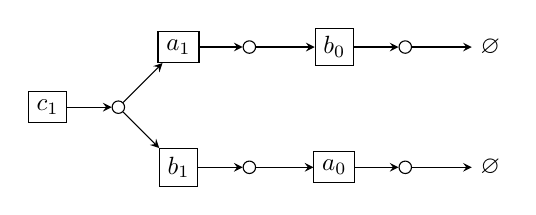
\begin{tikzpicture}[aS,every node/.style={scale=0.9}]  
  	\startl{c_1};
  	\specl{above}{c_1}{a_1};
  	\link{a_1}{b_0};
  	\edl{b_0};
  	\specl{below}{c_1}{b_1};
	\link{b_1}{a_0};
  	\edl{a_0};
\end{tikzpicture}
\end{minipage}
\caption{The ABAN and the SLCG of example 2}
\label{fig:3}
\end{figure}
In \textit{Example \ref{example:reach}}, $a_1$ is reachable, while in \textit{Example \ref{example:unreach}}, $c_1$ is unreachable. This inconclusiveness is a limitation of SLCG as $r'(\alpha,\omega)$ is not equivalent to $reach(\alpha,\omega)$.

As there are cycles in SLCG generated by feedback loops in biological regulatory networks, the existing approach does not allow a solution generally.

%Even though we broadened the applicability of SLCG, this method is still not universally applicable for all ABANs or BNs due to the limitations. 
From the former examples, we realize that it is difficult to solve the reachability problem in general. 
In the rest of this paper, we are going to discuss how to improve the performance of existing approaches and our new methods. 

\section{Heuristics for inconclusive cases}\label{sect:4}
SLCG loses its generality of solution due to the existence of AND gates.
In this section, we are trying to make a little compromise in exactitude in order to have a general solution of reachability problem. 
As a consequence, the out-degree of corresponding AND gates in SLCG is bounded to $O(1)$.
This hypothesis is reasonable, because in ordinary biological networks, every component interacts only with a small part of the whole network \cite{akutsu2007control}.
To face with an arbitrary ABAN in this context, for now, the remaining tasks are cycles and conflicts in its SLCG.
\subsection{Preprocessing of SLCG}\label{sectprecond}
\subsubsection{Detection of cycles}
The notion of cycle can be expanded to Strongly Connected Components (SCC) of size greater than 1 as an SCC may contain several nested cycles. 
In \cite{tarjan1972}, the search of SCCs can be done in $O(|V|+|E|)$ time. 
%As SLCG is in fact a sparse graph (the out-degree is limited to $O(1)$), the search of SCCs can be done in $O(|V|)$, \textit{i.e.} linear time.

\subsubsection{Removing cycles}
\begin{theorem}\label{cycletheo}
Given a cycle, if it contains no OR gate% towards outside of cycle
, all the local states in the cycles are unreachable.
\end{theorem}

\begin{proof}
Suppose an arbitrary cycle $C=a_i\mapsto \cdots b_j\mapsto\cdots \mapsto a_i$, with $\mapsto$ an edge in the SLCG.
Note that $r'(\alpha,a_i)\implies r'(\alpha,b_j)\implies r'(\alpha,b_j.\text{next})\implies \cdots\implies r'(\alpha,a_i)$.
According to the definition of $r'$, $r'(\alpha,a)=\mathbf{True}$ only if $\exists c_k\in C$ and $c_k\in \alpha$.
If there exists such $c_k$, $C$ should not exist as the reasoning stops at $c_k$ and does not form a cycle, contradiction.
$r'(\alpha,a_i)=r'(\alpha,b_j)=\cdots =\mathbf{False}$.\qed
\end{proof}

With Theorem \ref{cycletheo}, before stepping into the next part of dealing with AND gates, we can perform a recursive preprocessing by deleting the cycles in SLCG to ensure no cycle remaining.

\subsection{AND Gates in SLCG}\label{sectAndGates}
After preprocessing, we can get rid of cycles.
The next step is to analyze an SLCG with only AND gates.
To achieve this goal, we need to find a trajectory reaching all the components of the given AND gates simultaneously.
These components form a joint state, and if the joint state is reachable, the corresponding transition of AND gate can be fired. 

In Fig \ref{fig:1}, $s=\{ b_1,c_1\}$ is a joint state, when $s$ is reached, transition \ac{b_1,c_1}{a_0}{a_1} is firable.
As the cycles there are no cycles, the order reaching the members in a joint state is the only factor that affects the final reachability. 
The reachability of a joint state can be then formulated as sequential reachability:
\begin{definition}[Sequential reachability]
Let joint state $s=\{ls_1,\ldots,ls_n\}$, $p_1\ldots p_n$ is an arbitrary order of $1\ldots n$ and sequence $seq=ls_{p_1}::\ldots::ls_{p_n}$, sequential reachability of $seq$ is denoted $reach(\alpha,seq)=reach(\alpha,ls_1)::\ldots::reach(\alpha,ls_n)$.
From initial state $\alpha$, $s$ is reachable in the order $seq$ by following the trajectories given by SLCG.
\end{definition}

\begin{example}
Fig \ref{fig:5} shows the SLCG for reachability of $c_1$ in ABAN with transitions $\mathbf{T}=\{\acm{a_1,b_1}{c_0}{c_1},\acm{b_0}{a_0}{a_1},\acm{c_0}{b_0}{b_1}\}$.
\end{example}
\begin{figure}[ht]
\centering
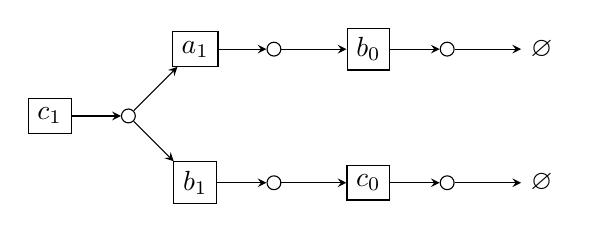
\begin{tikzpicture}[aS]  
  	
  	\startl{c_1};
  	\specl{above}{c_1}{a_1};
  	\link{a_1}{b_0};
  	\edl{b_0};
  	\specl{below}{c_1}{b_1};
	\link{b_1}{c_0};
  	\edl{c_0};
    \end{tikzpicture}

\caption{Reachability depends on firing order}
\label{fig:5}
\end{figure}

$a_1$ and $b_1$ are reachable respectively but is not necessarily for $c_1$.
If we begin with the branch with $a_1$, $s=\{a_1,b_1\}$ is reachable with trajectory $\acm{b_0}{a_0}{a_1}::\acm{c_0}{b_0}{b_1}::\acm{a_1,b_1}{c_0}{c_1}$. 
However if we begin with the branch $b_1$, after firing $\acm{c_0}{b_0}{b_1}$, $b_0$ is no longer reachable, resulting the unreachability of $a_1$.
We have $reach(\alpha,a_1::b_1::c_1)=\mathbf{True}$ and $reach(\alpha,b_1::a_1::c_1)=\mathbf{False}$.

As the firing order matters, we come to verify all the possible sequential reachabilities of certain joint state to obtain its reachability.

\begin{proposition}\label{theoperm}
Given joint state $s=\{ls_1,\ldots,ls_n\}$, with all the local states in $s$ are reachable: $reach(\alpha,ls_i)=\mathbf{True},\ \forall i\in[1,n]$, the set of permutations of $s$ is denoted $Perm(s)=\{(ls_1::ls_2,::\ldots ::ls_n),\ \cdots,\ (ls_n::ls_{n-1}::\ldots,::ls_1)\}$. $\bigvee reach(\alpha,Perm(s))=\mathbf{True}$ is a necessary condition of $reach(\alpha,s)=\mathbf{True}$.
\end{proposition}
\begin{proof}
Notation: $a_i\triangleright b_j$ means that $a_i$ must appear before $b_j$.

Necessity: if there exists a permutation $perm_i\in Perm$ s.t. $reach(\alpha,perm_i)=\mathbf{True}$, then $s$ can be reached according to $perm_i$.
To reach $s$, every local state in SLCG is mandatory to be reached.
Given $\bigvee reach(\alpha,Perm(s))=\mathbf{False}$, does there exist a permutation $perm(Ls)$ s.t. $reach(\alpha,s)=\mathbf{True}$?

For solvable conflicts, $perm(s)$ probably covers one of the admissible order.
One possible counterexample is shown in Fig. \ref{FigConflictInForks}.
\qed\end{proof}

It is remarkable that the former approach is efficient in deciding reachability and finding reaching trajectory, but it has a drawback: if there exists a solvable conflict in different forks, traversing permutations may be not able to find the trajectory towards goal state.
In Fig \ref{FigConflictInForks}, if $sol_{c_1}$ is resolved first, automaton $d$ will be on state $d_1$, which disables the reachability of $b_1$.
In other cases, the trajectory of $a_1$ is retrievable.
\begin{figure}[ht]
\centering
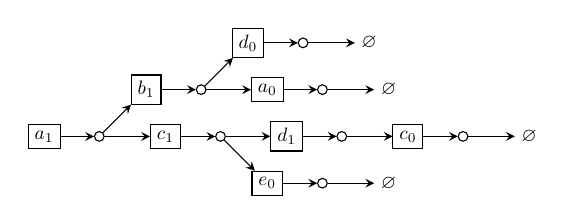
\begin{tikzpicture}[aS, every node/.style={scale=0.7}]  
  	
	\startl{a_1};
	\specl{above}{a_1}{b_1};
	\specl{above}{b_1}{d_0};
	\edl{d_0};
	\link{b_1}{a_0};
 	\edl{a_0};
	\link{a_1}{c_1};
 	\link{c_1}{d_1};
 	\link{d_1}{c_0};
 	\edl{c_0};
 	\specl{below}{c_1}{e_0};
 	\edl{e_0};
    \end{tikzpicture}
\caption{Conflicts in different forks}\label{FigConflictInForks}
\end{figure}

However there is more than one AND gate in general biological networks and those AND gates could be chained \textit{e.g.} \cite{samaga2009logic}, \textit{i.e.} the successors of certain AND gate contain other AND gates.
We analyze first the simple AND gates $simp$ (without successive AND gates) by traversing its permutations.
If all elements in $simp$ are reachable, update initial state by firing all the transitions and delete the successors of $simp$, then restart the process from finding simple AND gates.
During the whole process, if an AND gate is not reachable after traversing its permutations, the final goal state is not reachable as the SLCG is linked by logical AND. 
Otherwise, when the process terminates, there is no AND gate, SLCG is conclusive as there is no cycle or conflict.

%The statement above is the worst case: in reality, all AND gates are not necessarily composed of exact $I$ components, and permutations are determined to be unreachable before verification as its subsets may have been confirmed unreachable in other tentatives.

For example: given an AND gate $sol_a=b\land c\land d$, where $b,c,d$ are local states.
Normally 6 realizing orders need checking: $b::c::d$, $b::d::c$, $c::b::d$, $c::d::b$, $d::b::c$ and $d::c::b$. 
If we find the order $b::c$ is not realizable when verifying the first realizing order, then we do not have to verify the reachability of $b::c::d$ and $b::d::c$ where $b$ occurs before $c$. $d::b::c$ is not included, because firing $d$ changes its state before firing $b::c$.


\subsection{Heuristic on OR gates}\label{sec:OR}
In the previous section, without OR gates (one state node has multiple solution successors), reachability problem is solvable in polynomial time.
As every \textbf{OR gate} has multiple choices, to avoid combinatorial explosion, we use a simple heuristic: 
choose randomly one assignment for each trial.
Then we can construct a new LCG without \textbf{OR gate}, every state node has exactly one successive solution node.
In fact, if the desired state is reachable, it is probable that exact solution is found during the trial because there are more than one choice that makes the desired state reachable.

\subsection{Overall Process}\label{sectOverall}
Combining all the parts, the whole process of PermReach is shown as follows:
\begin{enumerate}
\item Precondition initial SLCG, cycles are deleted (Section \ref{sectprecond})
\item Build decision trees for AND gates and OR gates
\item Launch the heuristic on OR gates, obtain an SLCG with pure AND gates 
\item Tackle ABAN with AND gates, if reachable, quit; if not, return to step 3 
\end{enumerate}

\section{Implementation and Benchmarks}\label{sect:5}
The overall process in section \ref{sectOverall} is implemented in Python\footnote{Implementation and testing data sets are available at \url{https://github.com/XinweiChai/LCG-in-ASP}}. 
To evaluate the performance in large \textit{in silico} networks, we take T-cell Receptor model (TCR) \cite{saez2007logical} and epidermal growth factor receptor model (EGFR) \cite{samaga2009logic} as examples, with the former one containing 95 components and 206 transitions and the latter one containing 104 components and 389 transitions respectively. 

These models are originally Boolean networks.
According to Appendix \ref{appendix:C}, they are transformable to ABANs. We then take several automata as input, varying exhaustively their initial states combinations ($2^{init\_state}$), take the reachability of the states of another automata set as output.
We first test the performance of traditional model checkers, Mole\footnote{\url{http://www.lsv.fr/~schwoon/tools/mole}} and NuSMV\footnote{\url{http://nusmv.fbk.eu}}, in which Mole turns out to be timeout for 6 in 12 outputs, and all timeout for NuSMV in model EGFR.
Due to the big state space, traditional model checkers are not effective. 

To validate our approach, we first use a small model: phage-$\lambda$ model \cite{thieffry1995dynamical} to compare with an alternative reachability analyzer Pint \cite{pauleve2012}. In this model with 4 components and 12 transitions (without taking consideration of the self-regulations), our result shows complete conclusiveness while Pint is not able to figure out the reachability of $[cll=1]$. 
In big examples TCR and EGFR,
%Folschette \textit{et al.} using Pint \cite{folschette2015},
although PermReach takes more time than Pint, it outputs the sequence from initial state towards final state.
More importantly, it gives conclusive reachability for any input. 
In the TCR tests, PermReach gives exactly the same result as Pint did. As for EGFR tests, PermReach takes the inconclusive cases of Pint as input, and returns conclusive outputs.

%in his paper, there are about Almost all the examples in this paper are ``inconclusive'' in Pint, but they are solvable \textit{via} the presented heuristic technique. In \cite{folschette2015}, Folschette \textit{et al.} ran tests over the possible variations of 13 input nodes (different initial states), and observed the reachability of other 12 components. In total $12\times 2^{13}=98,304$ instances are tested. Among these tests, there are 9,986 (10,16\%) inconclusive instances. We conducted tests on these instances and found out they are conclusive in our methods.

\begin{table}[ht]
\centering
    \begin{tabular}{|c|c|c|c|c|c|c|}
    \hline
  	Model	&\multicolumn{2}{c|}{$\lambda$-phage}	&	  \multicolumn{2}{c|}{TCR} & \multicolumn{2}{c|}{EGFR}  \\
    \hline
    Inputs&\multicolumn{2}{c|}{4}	&	  \multicolumn{2}{c|}{3} & \multicolumn{2}{c|}{13}\\
    \hline
    Outputs&\multicolumn{2}{c|}{4} &	  \multicolumn{2}{c|}{5} & \multicolumn{2}{c|}{12} \\
    \hline
    Total tests&\multicolumn{2}{c|}{$2^4\times 4=64$} & \multicolumn{2}{c|}{$2^3\times 5=40$} & \multicolumn{2}{c|}{$2^{13}\times 12=98,304$}\\
    \hline
    Analyzer  &  Pint       &\textbf{PermReach}    &  Pint       &\textbf{PermReach}   &  Pint       &\textbf{PermReach}             \\
    \hline
    Reachable    & 36(56\%)& 38(59\%)   &  \multicolumn{2}{c|}{16(40\%)}  & 64,282(65.4\%)&74,268(75.5\%)\\
    \hline
    \textbf{Inconclusive} & \textcolor{red}{\textbf{2(3\%)}}&\textcolor{blue}{\textbf{0(0\%)}}& \multicolumn{2}{c|}{0(0\%)}    &\textcolor{red}{\textbf{9,986(10.1\%)}}&\textcolor{blue}{\textbf{0(0\%)}}  \\
    \hline
    Unreachable     &  \multicolumn{2}{c|}{26(41\%)} &  \multicolumn{2}{c|}{24(60\%)} &24,036(24.5\%)&24,036(24.5\%)\\
    \hline
    Total runtime &  $<1$s       &  $<1$s &  \textbf{7s}       &  \textbf{0.85s}        & \textbf{9h50min}              & \textbf{15min31s}      \\
    \hline
    \end{tabular}
\caption{Results of the tests on large-scale examples using Intel Core i7-3770 CPU, \@3.4GHz, 8.00G RAM. 
Column “Pint” gives the related results on ANs, while column “PermReach” gives the results for ABANs. 
“True”, “Inconclusive” and “False” give respectively the number of different results of reachability, while “Max time” and “Total time” depict respectively the maximum time of the individual computations.}
\label{tab:2}
\end{table}

We carried some random tests\footnote{Random ABANs are generated as follows: given the number of transitions, for every transition, the head of the }, with the number of automata varying from $10,20,\ldots,100,200,\ldots,1000$.
We varied also the density of the transitions (transitions per automaton on average) from 1 to 10.
Results of small examples are validated by traditional model checker as it always gives exact result.

As seen in the previous results, our heuristic technique is more conclusive than the reasoning of Pint. 
In the configuration of the heuristic approach, if there are less than 20 OR gates after preprocessing in Section \ref{sectprecond}, the computation will be shifted from heuristic to global search as the size of enumeration is acceptable.
There are only 11 OR gates in EGFR model, therefore the results are firmly conclusive. 


To sum up, PermReach has a better time performance than traditional exhaustive model checkers (Mole and NuSMV); on the other hand, it is more conclusive than abstract analyzers (Pint) while keeping a reasonable time performance.

\section{Conclusion and future work}\label{sect:6}
This paper proposes an expressive formalism ABAN to study the reachability problem. 
The original approach SLCG has limited conclusiveness because static and local reasoning does not simulate all real system dynamics. 
Due to the complexity of global search, developing a heuristic technique based on joint states becomes a feasible choice.
The heuristic method reproduces the system dynamics by traversing possible orders of transitions. 
This ``dynamic tentative'' makes it closer to real dynamics than LCG is.

Future work: in the reasoning of AND gates, the computation on permutations is expensive but is still not conclusive enough, see Fig \ref{FigConflictInForks}. 
To speed up the whole procedure and improve the conclusiveness, we plan to apply SAT (Satisfiability) solvers or Answer Set Programming (ASP) to refine the analysis of transition orders ($\triangleright$) in the same fork and those across forks. 
In addition, we may contemplate the extension of our heuristic technique to multivalued models.


\bibliographystyle{splncs04}
\bibliography{bib}   % name your BibTeX data base

\appendix
\section{Algorithm}\label{appendix:B}
The construction of an SLCG is realized by iterative updates:
\begin{algorithm}[ht]
\begin{algorithmic}
\State Initialization: 
$Ls\gets \{\omega\}$, $\mathbf{LS}\gets\{\omega\}$, $\mathbf{Sol}\gets \varnothing$
\While{$Ls\neq \varnothing$}
	\For{$a_i\in Ls$}
		\State $Ls\gets Ls\backslash a_i$
		\If{$a_i\in init\_state$}
			\State $a_i{\rm .next}=sol_{a_i}$
            \State $sol_{a_i}{\rm .next}=\varnothing$
    	\Else
    		\For{$sol=\acm{A}{a_{1- i}}{a_i}\in \mathbf{T}$}
    			\State $a_i{\rm .next}\gets a_i{\rm .next}\cup sol$
    			\For{$b_j\in A$}
    				\State $sol{\rm .next}\gets b_j$
    			\EndFor
    			\State $Ls\gets Ls\cup b_j$
                \State $\mathbf{LS}\gets \mathbf{LS}\cup Ls$
    		\EndFor
    		\State$\mathbf{Sol}\gets \mathbf{Sol}\cup a_i{\rm .next}$           
    	\EndIf
	\EndFor
\EndWhile
\State\Return{$(\mathbf{LS},\mathbf{Sol})$}
\end{algorithmic}
\caption{SLCG construction}
\label{algorithm:2}
\end{algorithm}
\section{Transformation from general BNs to ABANs}\label{appendix:C}

Given Boolean functions $v_i(t+1)=f_i(\mathbf{V}_i)$, with $\mathbf{V}_i$ the set of participating variables among $v_1(t),\cdots,v_n(t)$.
Boolean operators are transformable to the composition of $\lnot,\land,\lor$ (\textit{e.g.} $a\ \mathbf{XOR} \ b = (a\land \lnot b)\lor (\lnot a\land b)$), and Boolean functions possess an equivalent CNF (clausal normal form) thanks to its distributivity.
As ANs interpret transitions in the way of disjunctions of conjunctions, all BNs are transformable to ANs. 
We can see that it does not matter whether the dynamics is synchronous or asynchronous, because these transformations are only exerted on functions/transitions.

Example: 

Let $G_B=(V,F)$ a BN with $V=\{a,b,c,d,e\}$, and has only one Boolean function, $F=\{f(a)= (b\lor c)\land(d\lor e)\}$, we have 
$f(a)=(b\land d)\lor(b\land e)\lor(c\land d)\lor(c\land e)$, and $\lnot f(a)=(\lnot b\land \lnot c)\lor(\lnot d\land \lnot e)$. 
The equivalent ABAN is then constructed: 5 automata $\mathbf{\Sigma}=\{a,b,c,d,e\}$, with transitions: $\mathbf{T}=\{\acm{b_1,d_1}{a_0}{a_1},\ \acm{b_1,e_1}{a_0}{a_1},\ \acm{c_1,d_1}{a_0}{a_1},\ \acm{c_1,e_1}{a_0}{a_1},\ \acm{b_0,c_0}{a_1}{a_0},\ \acm{d_0,e_0}{a_1}{a_0}\}$.
\end{document}